% ! TeX root = ../../main.tex
\chapter{Implementazione}
In questo capitolo vengono trattati tutti gli aspetti ritenuti particolarmente interessanti durante la fase d'implementazione dell'applicativo TotemBoschettoAR\footnote{https://github.com/TeoV00/TotemBoschettoAR.git}, come l'uso di pattern, oltre a mostrare gli screenshot delle pagine sviluppate.

\section{Integrazione totem e app BoschettoAR}
L'integrazione fra il totem e l'app ha richiesto un'analisi sulla disponibilità e praticabilità di utilizzare determinate tecnologie per l'interazione fra i due dispositivi anche in un'ottica di \textit{user experience}, usabilità e scalabilità.

Per il trasferimento dei dati da app a totem è stato considerato l'utilizzo della tecnologia NFC ma la mancanza dell'hardware necessario, e considerando che non tutti gli smartphone (in particolare quelli meno recenti) possiedono tale tecnologia, si è deciso di non utilizzarla.

Come ulteriore alternativa per il caricamento dei progressi utente dall'app si è valutato di utilizzare un'architettura client-server con API esposte dal web-server installato sul totem. Quest'ultima opzione sarebbe stata un buon compromesso in termini di sicurezza e velocità di trasmissione ma poco scalabile e avrebbe limitato la condivisione dei dati a solo quegli utenti connessi alla rete WiFi della sede dell'Ateneo.

Viste le precedenti considerazioni si è optato per un'integrazione basata sul \textit{cloud computing} e, più precisamente, utilizzando come servizio \textit{cloud-based} per la memorizzazione in tempo reale dei dati Firebase Realtime di Google \cite{firebase} che offre, anche gratuitamente, scalabilità, affidabilità, facilità d'uso e sicurezza.
Scegliendo questo modo d'integrazione si apre la possibilità di aggiungere nel tempo nuove totem interattivi per l'espansione del progetto in altre sedi dell'Università di Bologna.

\section{Organizzazione progetto}
I file del progetto sono organizzati in cartelle relative a ciascuna schermata, componente o funzionalità. L'albero delle cartelle viene presentato nel listato \ref{lst:projectDir} dove vengono espanse solo le cartelle di primo livello (model, views e dataProvider). All'interno della cartella \texttt{model} sono state inserite le classi che definiscono il modello dei dati utente (file \texttt{share\_data\_model.dart}) e i metodi/classi/interfacce di utilità (file \texttt{obj2map.dart}), in \texttt{views} sono presenti i file delle schermate raccolti in cartelle e infine in \texttt{dataProvider} sono contenuti tutti i provider di dati utilizzati dal \texttt{DataManager} (file \texttt{data\_manager.dart}) per il reperimento delle informazioni.

\begin{lstlisting}[language=C, caption={Albero della directory del progetto TotemBoschettoAR}, label={lst:projectDir}]
    TotemBoschettoAR/
        |
        +- model/
            |
            +- obj2map.dart
            +- share_data_model.dart
        +- views/
            |
            +- common/
            +- navigation_menu/
            +- home_page/
            +- stats_page/
            +- chart_page/
            +- info_page/
            +- home_page.dart
            +- stats_page.dart
            +- chart_page.dart
            +- info_page.dart
        +- dataProvider/
            |
            +- firebase_provider.dart
        +- unit_converter.dart
        +- data_manager.dart
        +- main.dart
\end{lstlisting}
\break
\section{App Mobile}
Seguendo i mockup sono state sviluppate le diverse schermate per la condivisione dei progressi. Sono state effettuate alcune modifiche come si può notare dagli screenshot in figura \ref{fig:shareDataApp}: in sostituzione al nickname utente impostato è stata messa una breve indicazione, che si trovava precedentemente nella pagina di scansione, sul come visualizzare il QR code del totem e infine la schermata di caricamento è stata modificata sostituendo l'icona e mostrando un testo che informi l'utente del caricamento dei dati.
\begin{figure}[h!]
    \centering
    \subfloat[Pagina di condivisone progressi]{
        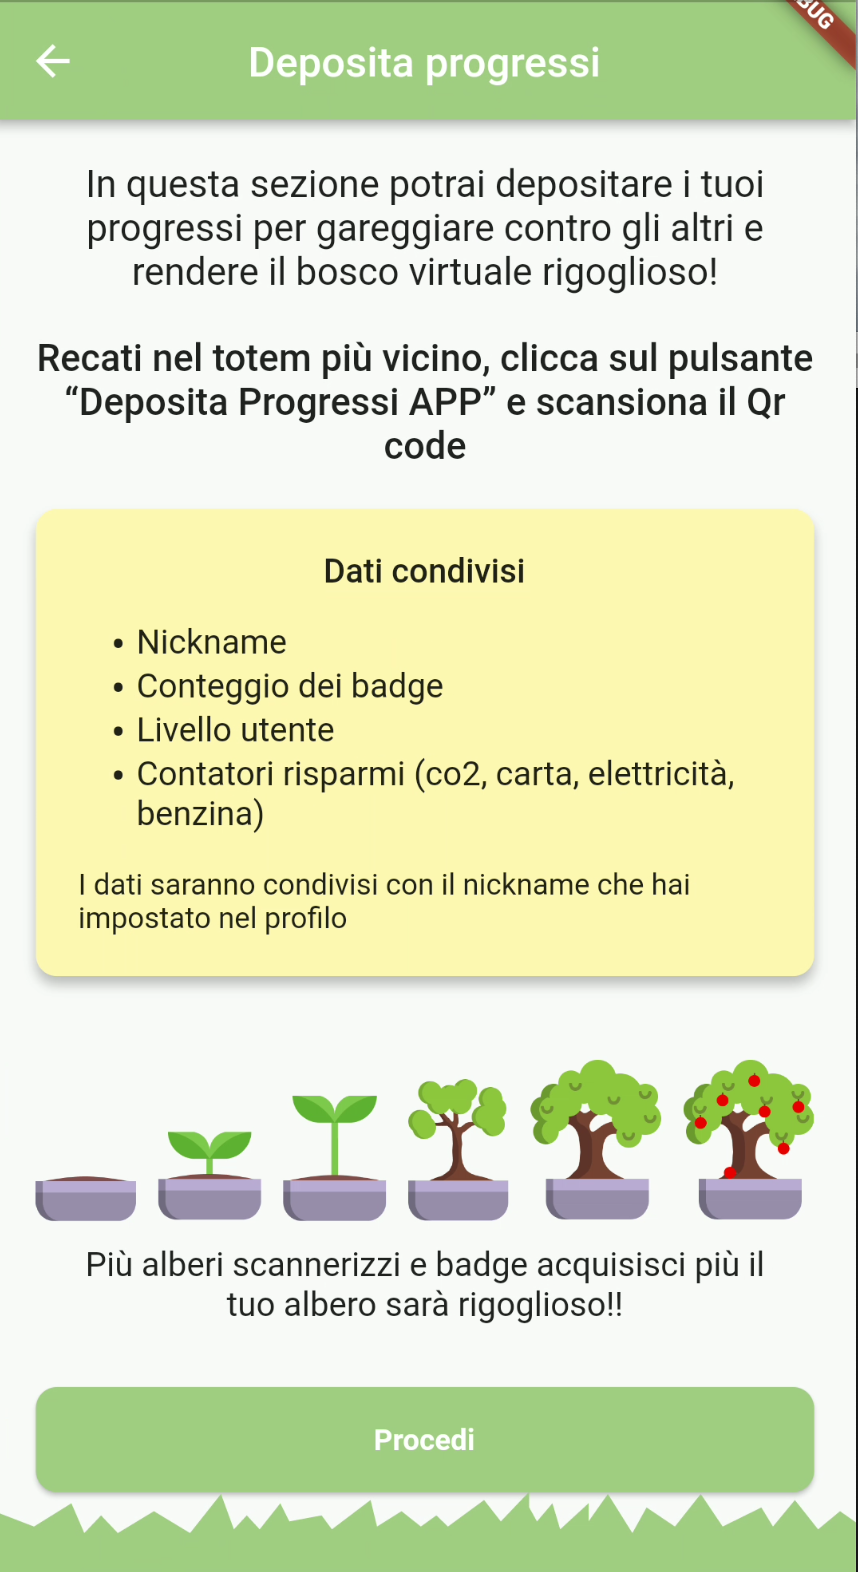
\includegraphics[width=0.3\textwidth]{img/app/uploadPage.png}
        \label{fig:sharePage}
    }
    \subfloat[Scansione QR code totem]{
        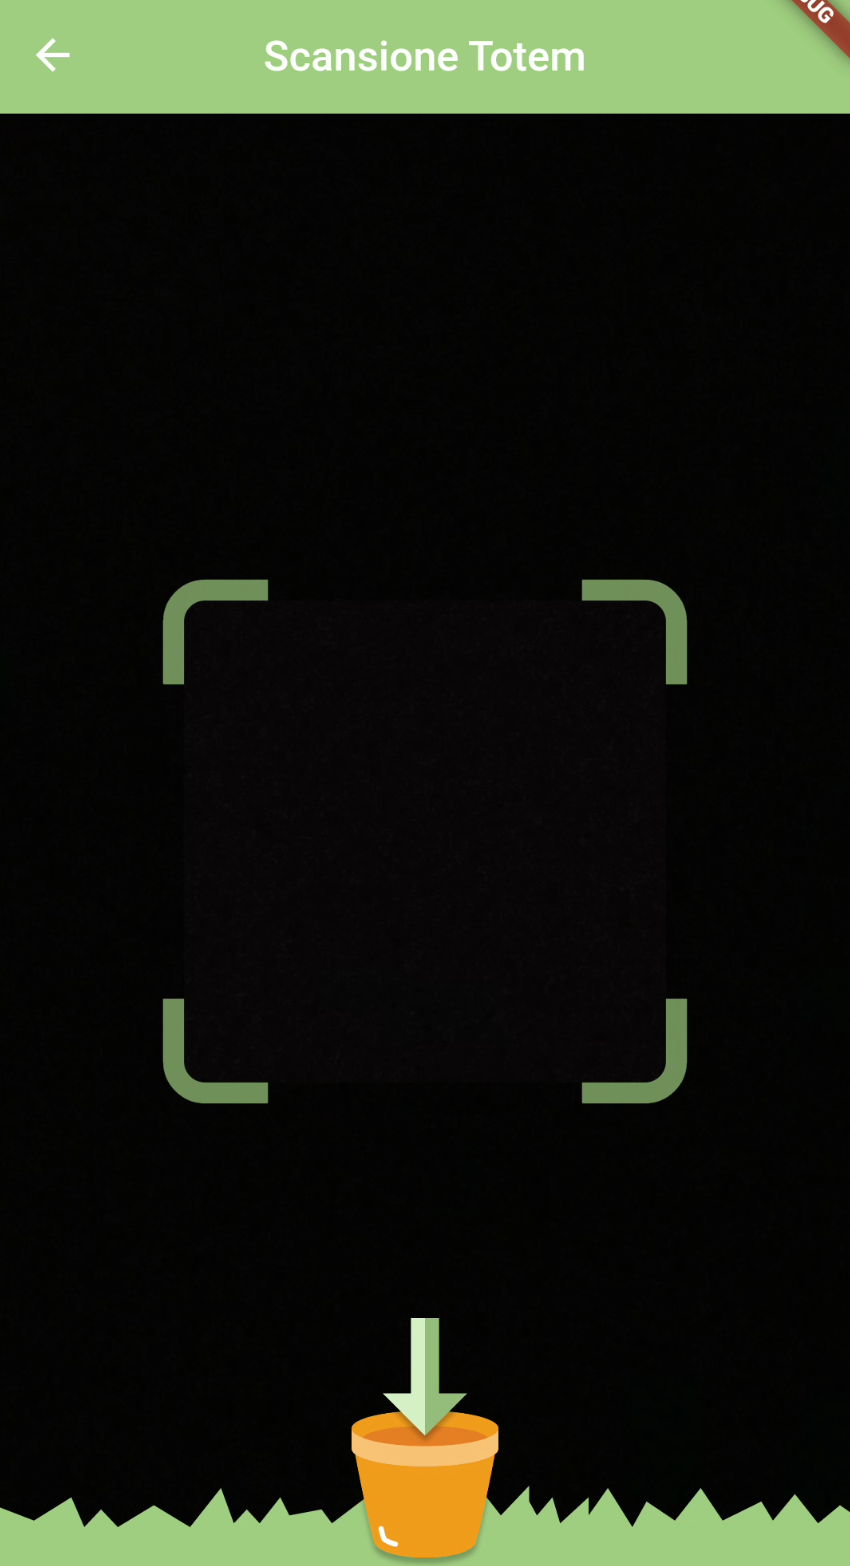
\includegraphics[width=0.3\textwidth]{img/app/uploadProgress.png}
        \label{fig:scanTotem}
    }
    \subfloat[Schermata di caricamento progressi]{
        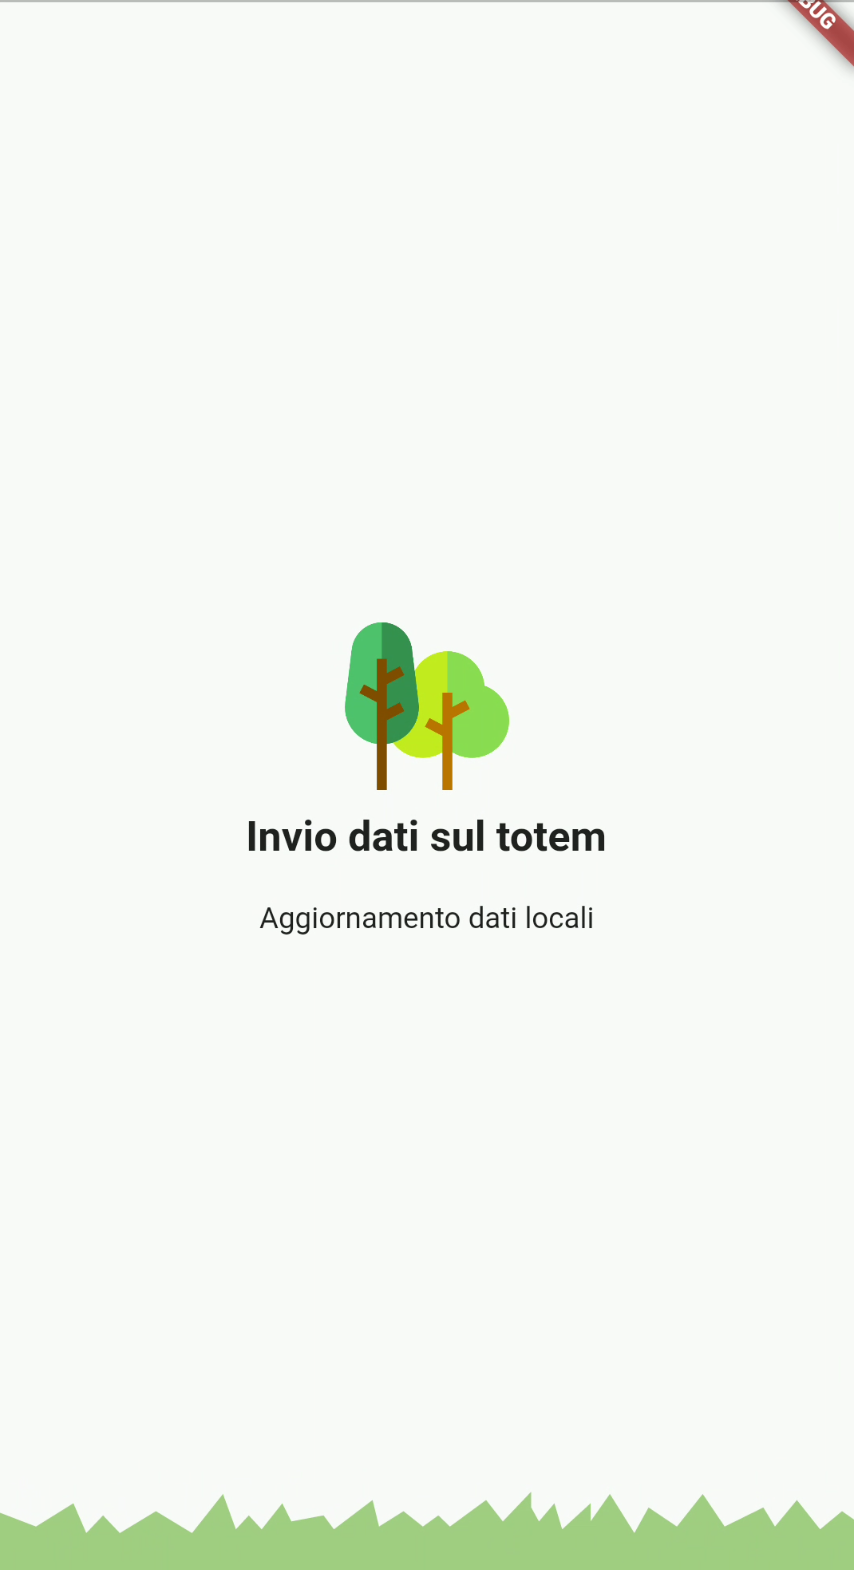
\includegraphics[width=0.3\textwidth]{img/app/uploadingPage.png}
        \label{fig:uploadinData}
    } 
    \caption{Screenshot schermate condivisione dati da app, scansione totem e caricamento \cite{repoBoschettoAR}}
    \label{fig:shareDataApp}
\end{figure}
\subsection{Pagina di condivisione progressi}
La schermata di caricamento dei progressi è raggiungibile dalla pagina utente oppure direttamente dalla pagina \textit{Home} in cui vi sono gli alberi collezionati. Nella barra degli strumenti (\texttt{AppBar}) di entrambe le pagine è stato aggiunto un pulsante (\texttt{IconButton}) che permette di aprire la pagina di condivisione aggiungendola allo stack di schermate dell'app chiamando il metodo \textit{push} della classe \texttt{Navigator} che disciplina la navigazione fra pagine. Nel listato \ref{lst:shareIconButton} da riga 7 a riga 20 inclusa viene mostrato il codice inserito.

\begin{lstlisting}[style=FlutterStyle, caption={Codice aggiornato della barra degli strumenti dell'app: inserito pulsante per la condivisione dei progressi.}, label={lst:shareIconButton}]
    Scaffold (
      backgroundColor: Colors.white,
      appBar: AppBar(
        centerTitle: true,
        backgroundColor: mainColor, 
        title: const Text("Profilo"),
        leading: IconButton(
          onPressed: () => Navigator.push(
            context,
            MaterialPageRoute(builder: (context) {
              return const SharePorgressPage();
            }),
          ),
          icon: const Icon(
            Icons.upload,
            size: 25,
            semanticLabel: "Carica progressi",
          ),
        ),
      ),
      body: //contenuto della pagina Utente o della Home
    );
\end{lstlisting}
\subsection{Scansione del QR code}
La schermata d'identificazione del totem tramite QR prevede il riutilizzo della classe \texttt{ScanQRView} che si occupa della grafica dello schermata, della gestione della fotocamera e del flusso dati generato dal riconoscimento di un codice QR; questa classe viene utilizzata anche dalla pagina di scansione dell'albero e in seguito ad una rifattorizzazione del codice, è stato applicato il pattern \textit{Strategy} in modo da poter decidere quale schermata mostrare dopo la scansione di un codice QR e soprattutto come gestire, validare e utilizzare i dati riconosciuti senza dover andare a creare tante versioni della classe \texttt{ScanQRView} specifiche. In figura \ref{fig:strategyQRScan} viene mostrato lo schema UML che chiarisce il ruolo delle classi all'interno del pattern \textit{Strategy}: la strategia è rappresentata dall'interfaccia \texttt{QrScanData} mentre le implementazioni sono la classe \texttt{SucessfullDataLoaded} (listato \ref{lst:SucessfullDataLoaded}) e la classe \texttt{ArViewLoader} rispettivamente per il caricamento dei progressi utente nel totem e per l'identificazione dell'albero.
\vspace{0.5em}
\begin{lstlisting}[style=FlutterStyle, caption={Codice rilevante della classe \texttt{SucessfullDataLoaded}.}, label={lst:SucessfullDataLoaded}]
class SucessfullDataLoaded implements QRScanData {
  String? data;

  @override
  Widget getWidget() {
      String totemId = data!;
      ... // codice omesso 
      Consumer<DataManager>(
        builder: (context, dataManager,_) => FutureBuilder<bool>(
          future: dataManager.uploadUserData(totemId)//intent
                             .timeout(UPLOAD_TIMEOUT),
          builder: (context, snap) {
            ConnectionState conState = snap.connectionState;
            bool uploadDone = snap.hasData ? snap.data! : false;
            if (conState == ConnectionState.waiting) {
              return const UploadingDataView();
            } else if (conState == ConnectionState.done) {
              if (uploadDone) {
                return const CompletedUploadView();
              } else {
                return const ErrorView(message: "Errore invio dati");
              }
            } else {
              return const ErrorView(message: "Errore sconosciuto");
            }
          },
        ),
      ),
      ... // codice omesso 
  }
  @override
  void setScannedData(String qrCodeData) {
    data = qrCodeData;
  }
}
\end{lstlisting}

\begin{figure}
  \centering
  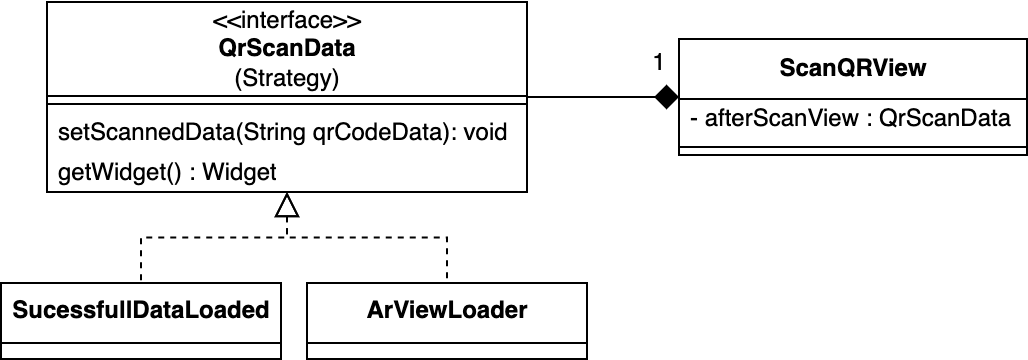
\includegraphics[width=10cm]{img/app/startegyScanQR.png}
  \caption{Pattern Strategy applicato alla scansione del codice QR nell'app mobile BoschettoAR}
  \label{fig:strategyQRScan}
\end{figure}
%%%%%%%%%%%%%%%%%%%%% TOTEM %%%%%%%%%%%%%%%%%%%%%%%%%%%%%%%%
\section{Totem}
\subsection{Dati Firebase}
Avendo deciso di utilizzare il database Firebase Realtime, che è di tipo documentale, è stato necessario convertire lo schema UML in figura \ref{fig:totemDomain} in formato JSON per avere la struttura generale dei dati che devono essere memorizzati.
Per ridurre il numero di oggetti annidati, si è deciso di separare le informazioni del totem (listato \ref{lst:totemInfo}) dai dati utente che sono stati condivisi tramite app (listato \ref{lst:userDataTotem}).

\begin{lstlisting}[language=json, caption={Esempio di oggetto JSON che memorizza i dati utente per ciascun Totem}, label={lst:userDataTotem}]
      "totems": {
        "totemId": {
          "userNickname": {
            "badgeCount": 0,
            "co2": 0,
            "level": 0,
            "nickname": "userNickname",
            "paper": 0,
            "treesCount": 0
          }
        }
      }
\end{lstlisting}
\break
\begin{lstlisting}[language=json, caption={Esempio di oggetto JSON contenente le informazioni sui totem}, label={lst:totemInfo}]
  "totemInfo": {
      "totemIdString": {
        "place": "locationName",
        "project": "projectName"
      },
    },
\end{lstlisting}  

\subsection{DataManager}
Il DataManager, come spiegato nel capitolo del design, funge sia da Repository che da Model del pattern MVI. Mantiene al suo interno i riferimenti ai diversi provider di cui fa uso, al momento solo \texttt{FirebaseProvider}, ed espone metodi che restituiscono degli \textit{State} indirizzati alla \textit{View} contenenti i dati richiesti dalle schermate. A livello implementativo gli \textit{State} sono oggetti della classe \texttt{Future} che è il tipo di dato di ritorno delle computazioni asincrone del \texttt{DataManager} e che, usato in combinazione con il \texttt{FutureBuilder}, permette di costruire l'interfaccia utente in base allo stato della computazione.

La classe \texttt{DataManager}, come si può notare in riga 1 del listato \ref{lst:dataManager}, estende \texttt{ChangeNotifier} e questo permette di aggiornare la View con i nuovi dati aggiornati appena modificati nel database.
Inoltre viene utilizzato il pattern Observer sul FirebaseProvider: il \texttt{DataManager}, implementando l'interfaccia \texttt{FirebaseObserver} e aggiungendosi come observer (riga 8 listato \ref{lst:dataManager}), viene notificato per qualsiasi genere di modifica dei dati nel cloud.
In cascata quindi ogni modifica sul database nel cloud fa scattare l'aggiornamento delle Views con il metodo \texttt{notifyListeners} (riga 24 listato \ref{lst:dataManager}).
\vspace{\baselineskip}
\begin{lstlisting}[style=FlutterStyle, caption={Classe DataManager}, label={lst:dataManager}]
class DataManager extends ChangeNotifier implements FirebaseObserver {
  final String _totemId = "ces_remade";
  late final FirebaseProvider _firebaseProvider;

  DataManager() {
    _firebaseProvider = FirebaseProvider(_totemId);
    _firebaseProvider.addObserver(this);
  }

  String getCurrentTotemId() {
    return _totemId;
  }

  Future<List<SharedData>> getData() async {
    return _firebaseProvider.getTotemData();
  }

  Future<List<SharedData?>> getTop10User() async {...}

  Future<Map<StatId, String>> getStatistics() async {...}

  @override
  void firebaseNotify() {
    notifyListeners(); 
  }
}
\end{lstlisting}
\newpage
\subsection{Pagina Home} 
Per la pagina principale è stata sviluppata l'idea del mockup in figura \ref{fig:forestHome} dove vengono visualizzate le chiome d'albero degli utenti che insieme compongono un bosco rigoglioso in quanto più affine all'idea di bosco virtuale e di comunità. 
Il pannello dei dettagli che si è scelto d'implementare è quello che ricorda una tendina con il cordino (figura \ref{fig:cordDetail}) in quanto ritenuto più adatto alla visualizzazione a chiome degli utenti.

In figura \ref{fig:homepage} viene mostrata un'istantanea della homepage mentre nel listato \ref{lst:homepageCode} è possibile consultare il codice che si occupa della disposizione degli alberi (a riga 8) e del loro comportamento al tocco (in riga 14).

Per questa pagina, come per le altre, è stata utilizzata sempre la stessa metodologia e architettura del codice per la loro creazione: con l'ausilio del \texttt{FutureBuilder} è stata sviluppata la View con la possibilità di gestire con maggiore semplicità ed astrazione l'invio degli \textit{Inten}s al Model (metodi della classe \texttt{DataManager}) e la ricezione degli \textit{State} di risposta.
\vspace{\baselineskip}
\begin{lstlisting}[style=FlutterStyle, caption={Parte del codice per la creazione del bosco della Homepage}, label={lst:homepageCode}]
  Consumer<DataManager>( // model
  builder: (context, dataManager, child) =>
      FutureBuilder<List<SharedData>>(
      future: dataManager.getData(), // intent
      builder: (context, state) { // state 
        if (state.hasData) {
          // widget per la disposizione a griglia delle chiome
          return GridView.count( // view
            crossAxisCount: 20,
            mainAxisSpacing: 10,
            crossAxisSpacing: 10,
            children: (state.data ?? []).map(
              (userDataTree) {
                return GestureDetector(
                  onTap: () {
                    setState(() {
                      userData = userDataTree;
                      showDetails = !showDetails;
                    });
                  },
                  // chioma dell'albero dell'utente
                  child: ForestTree(level: userDataTree.level),
                );
              },
            ).toList(),
          );
        } else {
          return const Center(
              child: CircularProgressIndicator(
            color: Color.fromRGBO(161, 204, 130, 1),
          ));
        }
      },
    ),
  ),
\end{lstlisting}
\begin{figure}[h!]
  \centering
  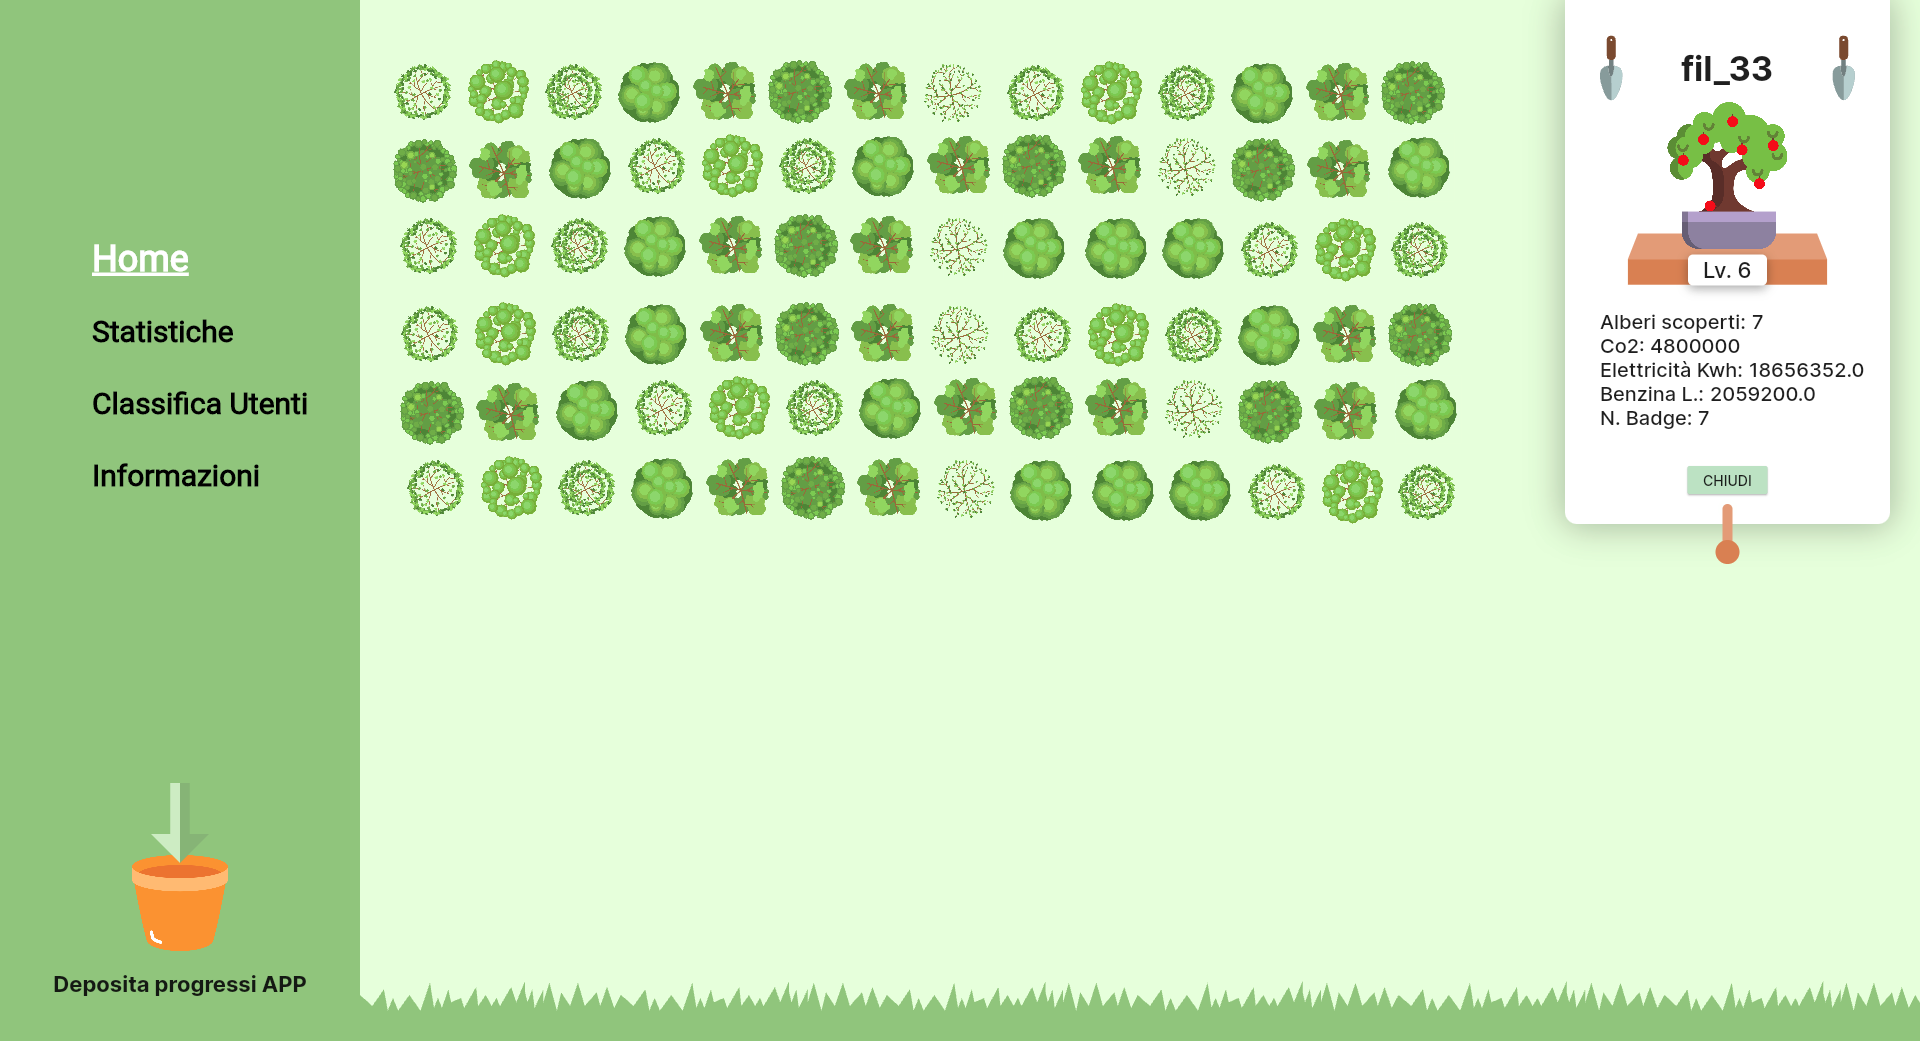
\includegraphics[width=\textwidth]{img/totem/screenshot/homepage.png}
  \caption{Screenshot della pagina Home dove viene visualizzato il bosco virtuale costruito dalla partecipazione degli utenti.}
  \label{fig:homepage}
\end{figure}
%
%
\break
\subsection{Pagina Statistiche}
Anche questa pagina (figura \ref{fig:statsPage}) prevede l'utilizzo delle classi \texttt{Consumer<DataManager>} e \texttt{FutureBuilder<DataManager>} per, rispettivamente, avere accesso al DataManager e poter richiedere e ricevere i dati statistici. Inoltre per la disposizione a griglia di sei colonne e tre righe dei contatori è stato utilizzato il costruttore \texttt{GridView.count}.
\begin{figure}[h!]
  \centering
  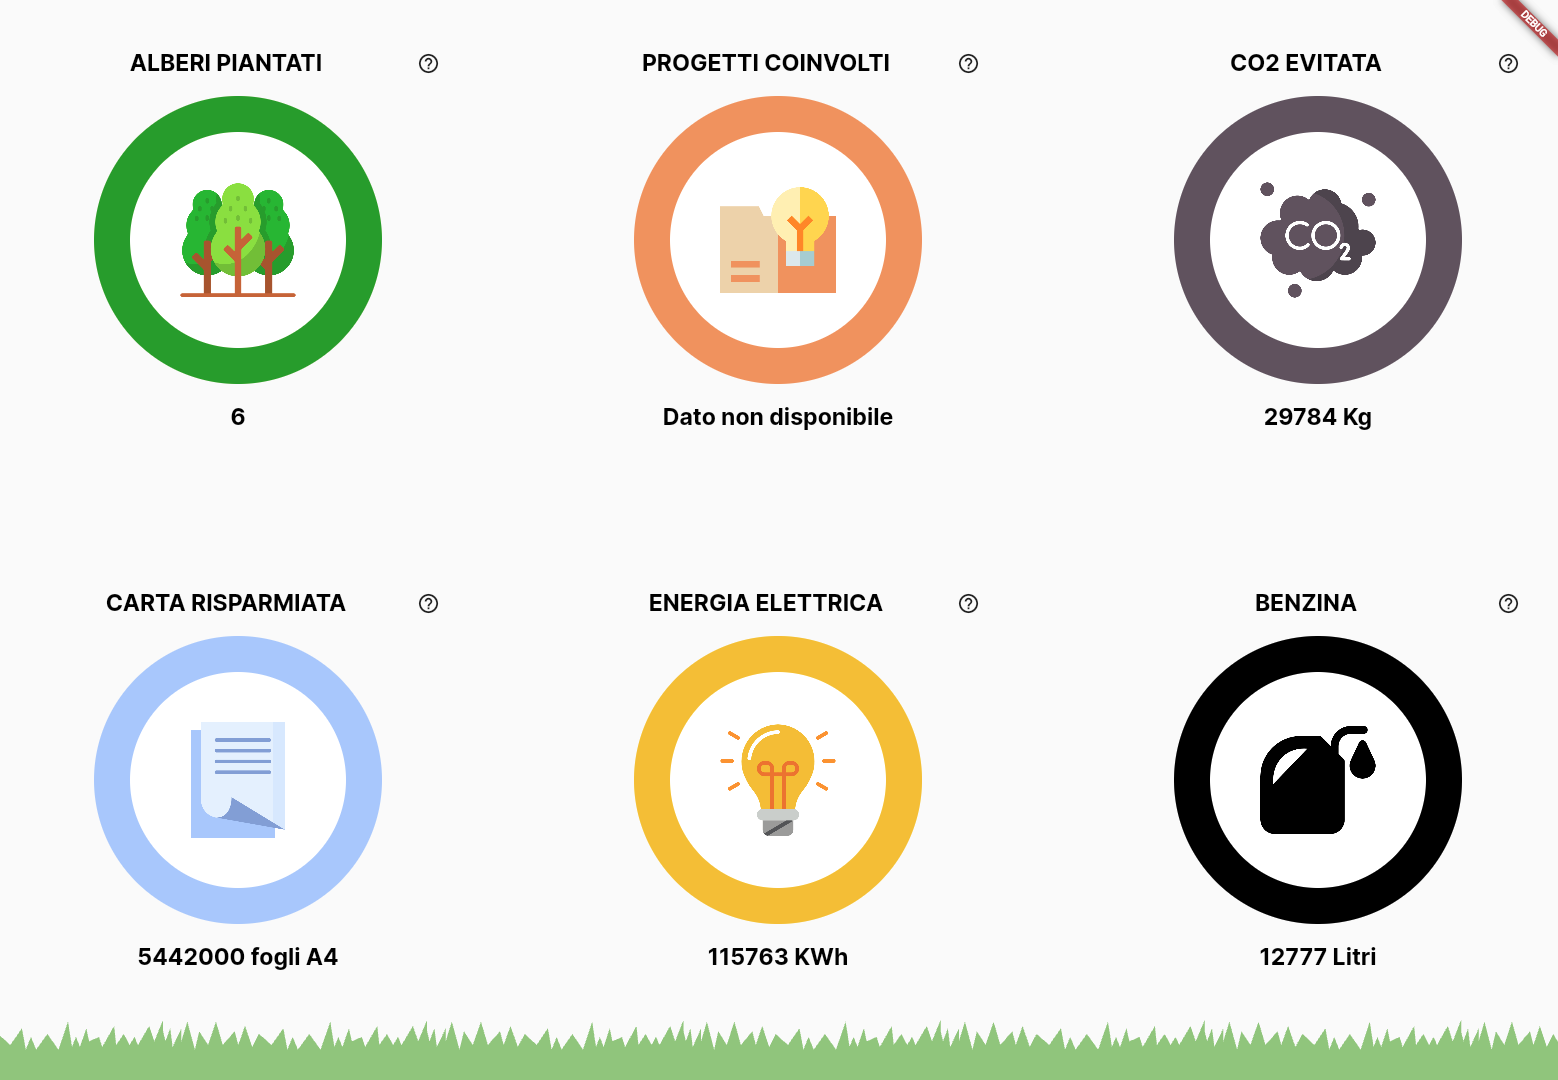
\includegraphics[width=\textwidth]{img/totem/screenshot/statsCircle.png}
  \caption{Pagina delle statistiche.}
  \label{fig:statsPage}
\end{figure}
\subsubsection{Contatore}
Il contatore è frutto della composizione di semplici elementi grafici sovrapposti fra di loro; osservando l'immagine \ref{fig:circleStat3d} partendo sinistra si ha un cerchio verde, uno bianco più piccolo, un'immagine e al di sotto una descrizione testuale. Al tocco i cerchi cambiano forma diventando quadrati, l'icona si sposta verso l'alto rimpicciolendosi e lasciando spazio al testo che viene mostrato.

I cerchi/quadrati vengono implementati (listato \ref{lst:roundedBox}) con la classe \texttt{RoundedBox} che restituisce un \texttt{AnimatedContainer}, un elemento grafico in grado di contenerne un altro e di generare un'animazione di se stesso quando viene modificato. Nel caso specifico del contatore viene modificato il raggio del bordo (\textit{borderRadius}) che passa da un valore massimo (cerchio) ad un valore di \texttt{10.0} (quadrato con spigoli smussati).

L'animazione dell'immagine è stata implementata (listato \ref{lst:resizingIcon}) utilizzando il \texttt{TweenAnimationBuilder} che sfrutta la generazione di valori compresi in un intervallo per la modifica della dimensione, insieme ad (\texttt{AnimatedSlide}) per la sua traslazione verso l'alto. Questa animazione è stata utilizzata anche nell'animazione della freccia nel pulsante per mostrare il codice QR del totem.

\vspace{\baselineskip}
\begin{lstlisting}[style=FlutterStyle, caption={Classe RoundedBox usata nella creazione del contatore delle statistiche}, label={lst:roundedBox}]
class RoundedBox extends StatefulWidget {
  final Color color;
  final double size;
  final double radius;

  const RoundedBox(
      {super.key,
      required this.color,
      required this.size,
      required this.radius});

  @override
  State<StatefulWidget> createState() => RoundedBoxState();
}

class RoundedBoxState extends State<RoundedBox> {
  @override
  Widget build(BuildContext context) {
    double size = widget.size;
    return AnimatedContainer(
      curve: Curves.ease,
      duration: const Duration(milliseconds: 400),
      width: size,
      height: size,
      decoration: BoxDecoration(
        color: widget.color,
        borderRadius: BorderRadius.all(Radius.circular(widget.radius)),
      ),
    );
  }
}
\end{lstlisting}
%
Infine per la descrizione del contatore (in figura \ref{fig:statCont3d} il rettangolo tratteggiato) è stata utilizzata la classe \texttt{AnimatedCrossFade}, incapsulata all'interno di \texttt{DescriptionBox} (listato \ref{lst:descrBoxStat}), che genera una transizione in dissolvenza tra \texttt{firstChild} e \texttt{secondChild}.
%
\vspace{\baselineskip}
\begin{lstlisting}[style=FlutterStyle, caption={Classe \texttt{ResizingIcon} che utilizza il \texttt{TweenAnimationBuilder}.}, label={lst:resizingIcon}]
  // animationStart e animationStop vengono invertiti in base a runTransition (booleano)
  TweenAnimationBuilder(
      tween: Tween<double>(begin: animationStart, end: animationStop),
      duration: widget.duration ?? defaultDuration,
      builder: (context, size, child) {
        return AnimatedSlide(
          duration: widget.duration ?? defaultDuration,
          offset: Offset(0.0, widget.runTransition ? widget.iconOffset : 0.0),
          child: SizedBox(
            height: size,
            width: size,
            child: widget.icon, // element a cui applicare l'animazione
          ),
        );
      },
    );
\end{lstlisting}
%
\begin{lstlisting}[style=FlutterStyle, caption={Stato della classe DescriptionBox che genera il widget della descrizione del contatore}, label={lst:descrBoxStat}]

  class _DescriptionBoxState extends State<DescriptionBox> {
    @override
    Widget build(BuildContext context) {
      var textBoxSize = widget.size - widget.boxPadding;
      return AnimatedCrossFade(
        firstChild: SizedBox(
          height: textBoxSize,
          width: textBoxSize,
          child: Padding(
            padding: EdgeInsets.all(widget.boxPadding) +
                (widget.offsetBox ?? const EdgeInsets.all(0)),
            child: Text(
              widget.description,
              style: TextStyle(fontSize: widget.textSize),
              textAlign: TextAlign.center,
            ),
          ),
        ),
        secondChild: const SizedBox(),
        crossFadeState: widget.showText
            ? CrossFadeState.showFirst
            : CrossFadeState.showSecond,
        duration: const Duration(milliseconds: 400),
      );
    }
  }
\end{lstlisting}
%
\begin{figure}[h!]
  \centering
  \subfloat[]{
    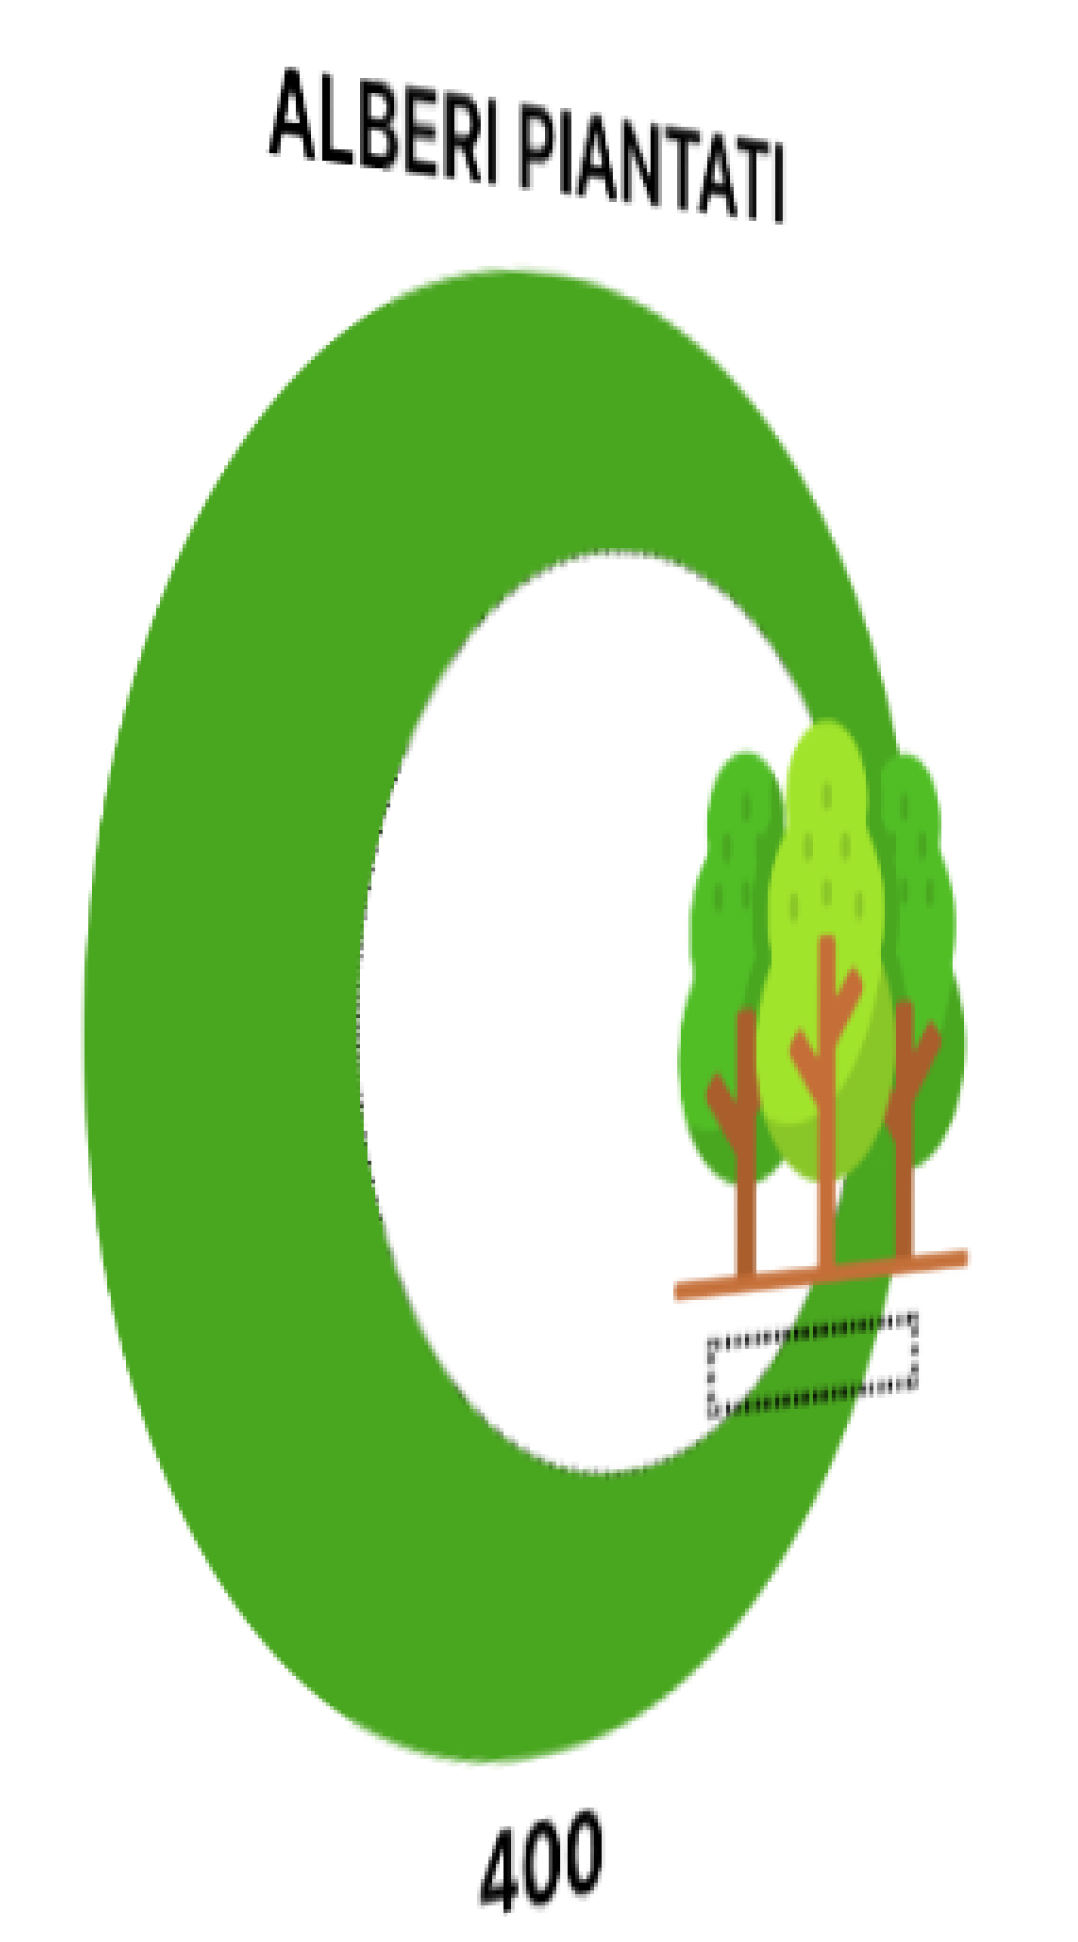
\includegraphics[width=3.5cm]{img/totem/circleStat3d.png}
    \label{fig:circleStat3d}
  }
  \subfloat[]{
    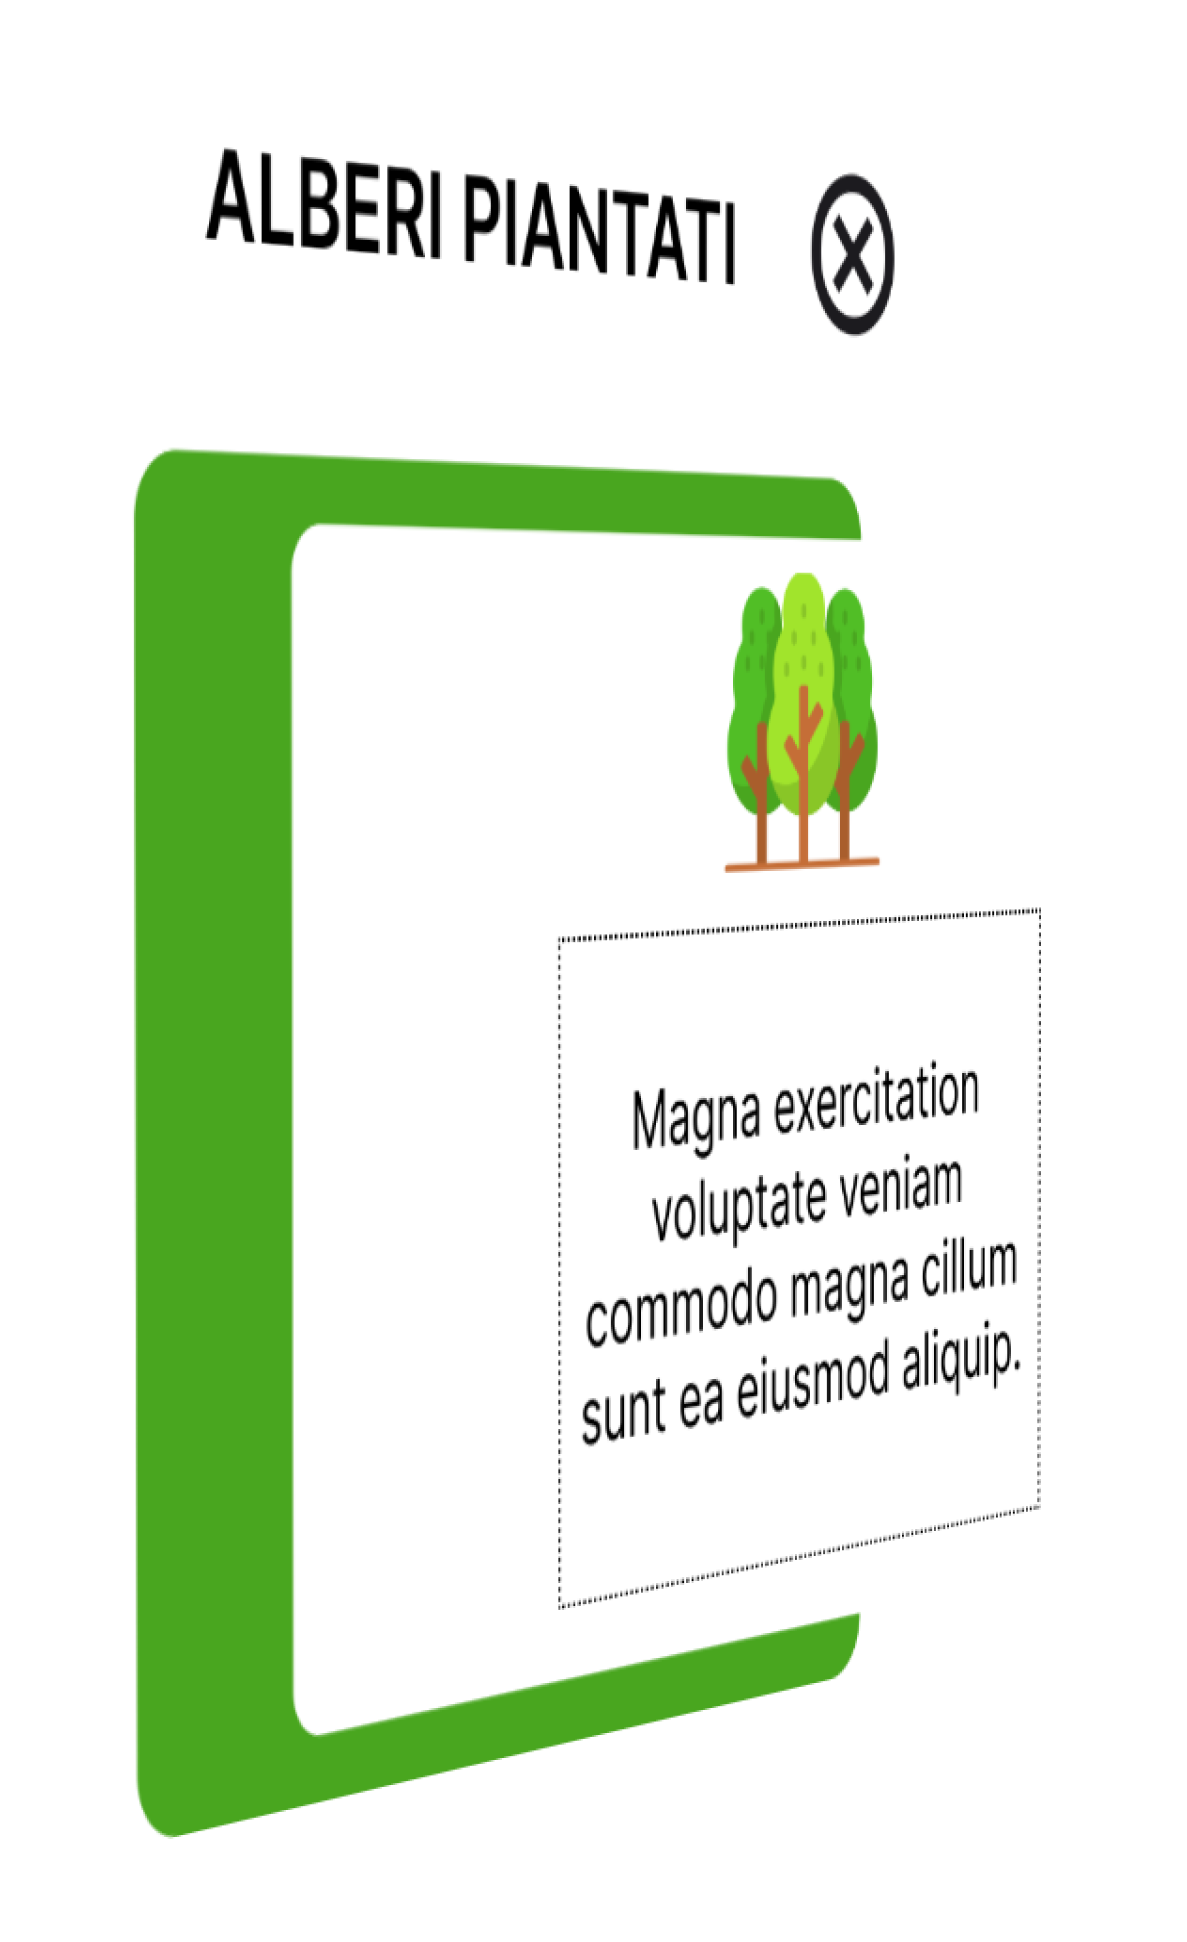
\includegraphics[width=4cm]{img/totem/squareStat3d.png}
    \label{fig:squareStat3d}
  }
  \caption[Contatore come composizione di widget]{Contatore delle statistiche come composizione di widget: un quadrato, con raggio del bordo variabile, all'interno dell'altro con sopra un'immagine e un testo (rettangolo tratteggiato).}
  \label{fig:statCont3d}
\end{figure}
%
%
\break
\subsection{Classifica}
Nella pagina della classifica (figura \ref{fig:top10screen}) rispetto al mockup, nelle diverse posizioni sono stati inseriti nuovi particolari grafici come la quantità di CO\textsubscript{2} e l'alberello che indica il livello utente in modo da renderli più interessanti e spronare ancora di più gli utenti a raggiungere il primo posto con un albero ricco di foglie e frutti.
\begin{figure}[h!]
  \centering
  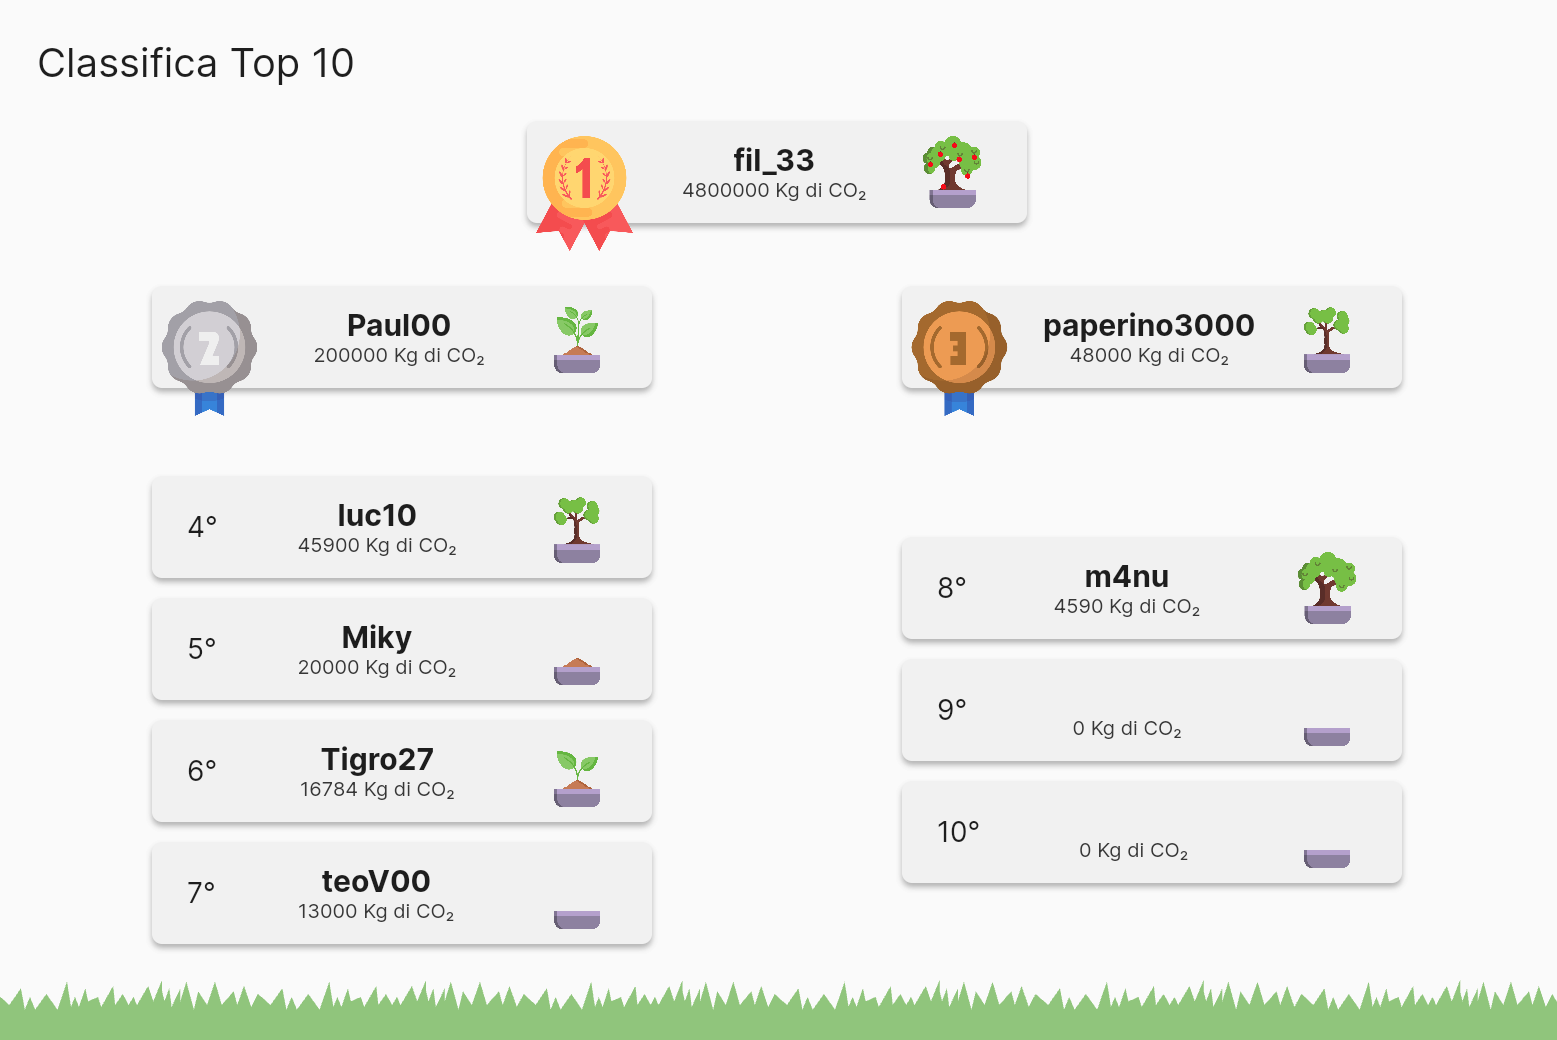
\includegraphics[width=\textwidth]{img/totem/screenshot/top10screen.png}
  \caption{Pagina della classifica conclusa.}
  \label{fig:top10screen}
\end{figure}

%
%
\subsection{Pagina Informazioni}
La pagina delle informazioni nel corso del suo concepimento ha subito vari cambiamenti, come anche precisato nel capitolo \ref{subsec:totem}, che comprendono un cambio drastico di layout passando da una semplice pagina scorrevole ad una visualizzazione a griglia contente tante \textit{tile}s (blocchi o piastrelle); la decisione d'implementare quest'ultimo layout è stata molto condizionata dall'esito di un sondaggio svolto su un piccolo gruppo di utenti target che, provando entrambi i mockup su device touchscreen, hanno dimostrato una maggiore preferenza per la visualizzazione a griglia in quanto più immediata, ordinata e di facile comprensione, prediligendo il tipo d'interazione \enquote*{con il tocco} (\textit{tap gesture}) per la fruizione delle informazioni al posto del prevalente scorrimento verticale (\textit{vertical scrolling gesture}). In figura \ref{fig:infoPage} viene mostrata la pagina delle informazioni e nella \ref{fig:infoPagePopup} una delle piastrelle espanse che mostra informazioni dettagliate.

Per la disposizione a griglia degli elementi è stato utilizzato il widget \texttt{GridView} (riga 6 listato \ref{lst:infoPageCode}) utilizzando un layout personalizzato definito dalla classe \texttt{SliverQuiltedGridDelegate} del package flutter \texttt{flutter\_staggered\_grid\_view} \cite{staggeredGridView} che permette agli elementi della griglia di occupare più righe e colonne.
Attualmente sono visualizzati cinque elementi di cui uno largo il doppio (figura \ref{fig:infopageLayout}) ma è possibile aggiungerne altri, di qualsiasi dimensione compatibile alla griglia, abilitando così la navigazione con scorrimento verticale.

\begin{lstlisting}[style=FlutterStyle, caption={Porzione di codice all'interno di \texttt{\_InfoPageState} per la creazione della pagina delle informazioni.}, label={lst:infoPageCode}]
  Stack(
    children: [
      Padding(
        padding: const EdgeInsets.all(50.0),
        // creazione vista a griglia
        child: GridView.custom(
          gridDelegate: SliverQuiltedGridDelegate(
            crossAxisCount: 3,
            mainAxisSpacing: 30,
            crossAxisSpacing: 30,
            repeatPattern: QuiltedGridRepeatPattern.inverted,
            pattern: const [
              // 1 riga ed 1 colonna occupata
              QuiltedGridTile(1, 1),  
              QuiltedGridTile(1, 1),
              QuiltedGridTile(1, 1),
              // 1 riga e 2 colonne occupate
              QuiltedGridTile(1, 2),
              QuiltedGridTile(1, 1),
            ],
          ),
          childrenDelegate: SliverChildBuilderDelegate(
            childCount: infoTiles.length,
            (context, index) => GestureDetector(
              child: Padding(
                padding: const EdgeInsets.only(bottom: 60.0),
                child: infoTiles[index],
              ),
              onTap: () {
                setState(() {
                  detailsWidget = infoTiles[index].getDetailsWidget();
                });
              },
            ),
          ),
        ),
      ),
      if (detailsWidget != null) ...[
        // pannello che mostra i dettagli relativi alla tile cliccata
      ],
    ],
  );
\end{lstlisting}
%
\begin{figure}[h]
  \centering
  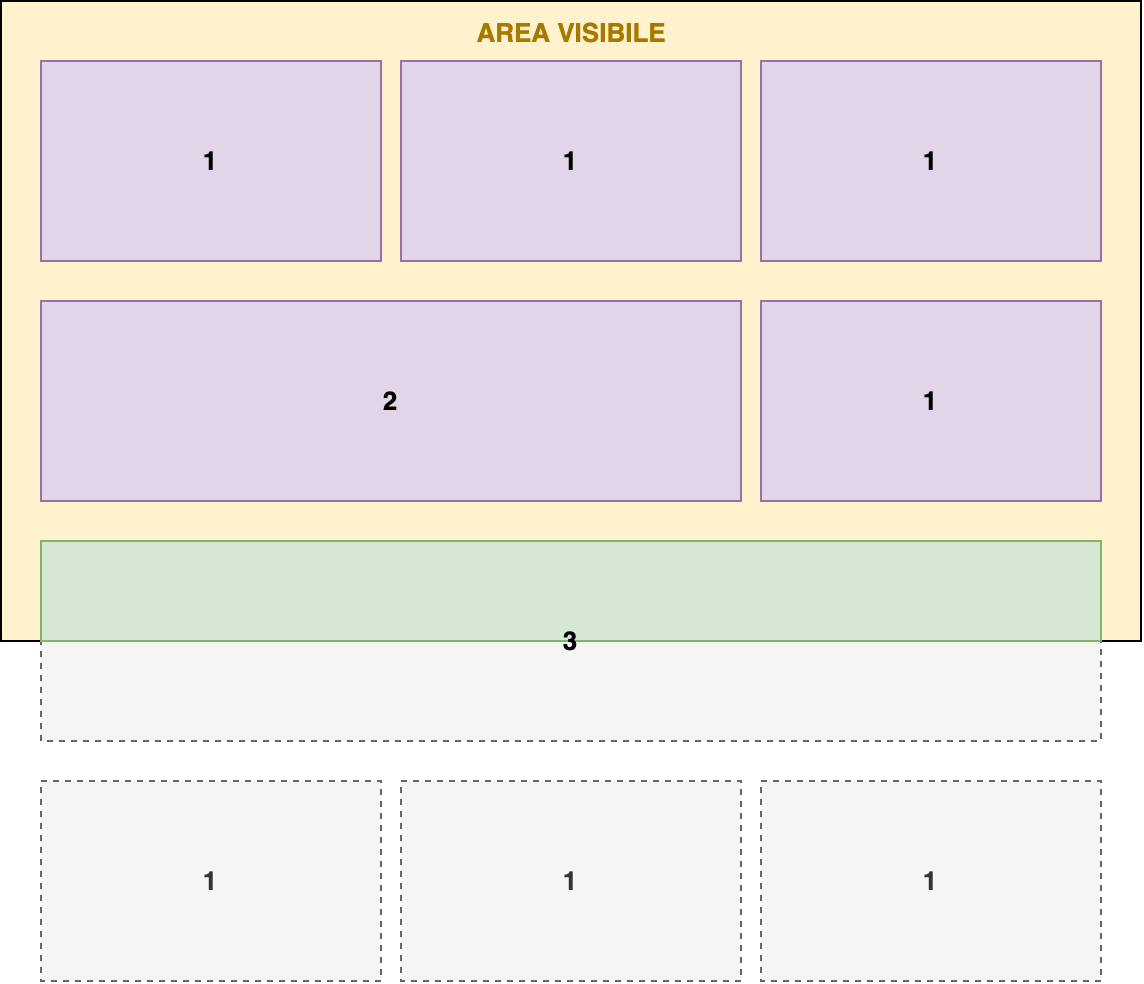
\includegraphics[width=9cm]{img/totem/layout_gridview.png}
  \caption[Layout pagina informazioni]{Layout pagina informazioni: in giallo l'area visibile, in viola le tile attualmente presenti infine in grigio quelle che potrebbero essere aggiunte, non esclusivamente in quella disposizione. I numeri presenti indicano quante colonne occupa ciascuna piastrella.}
  \label{fig:infopageLayout}
\end{figure}
%
\begin{figure}
  \centering
  \begin{minipage}[h]{0.9\linewidth}
    \centering
    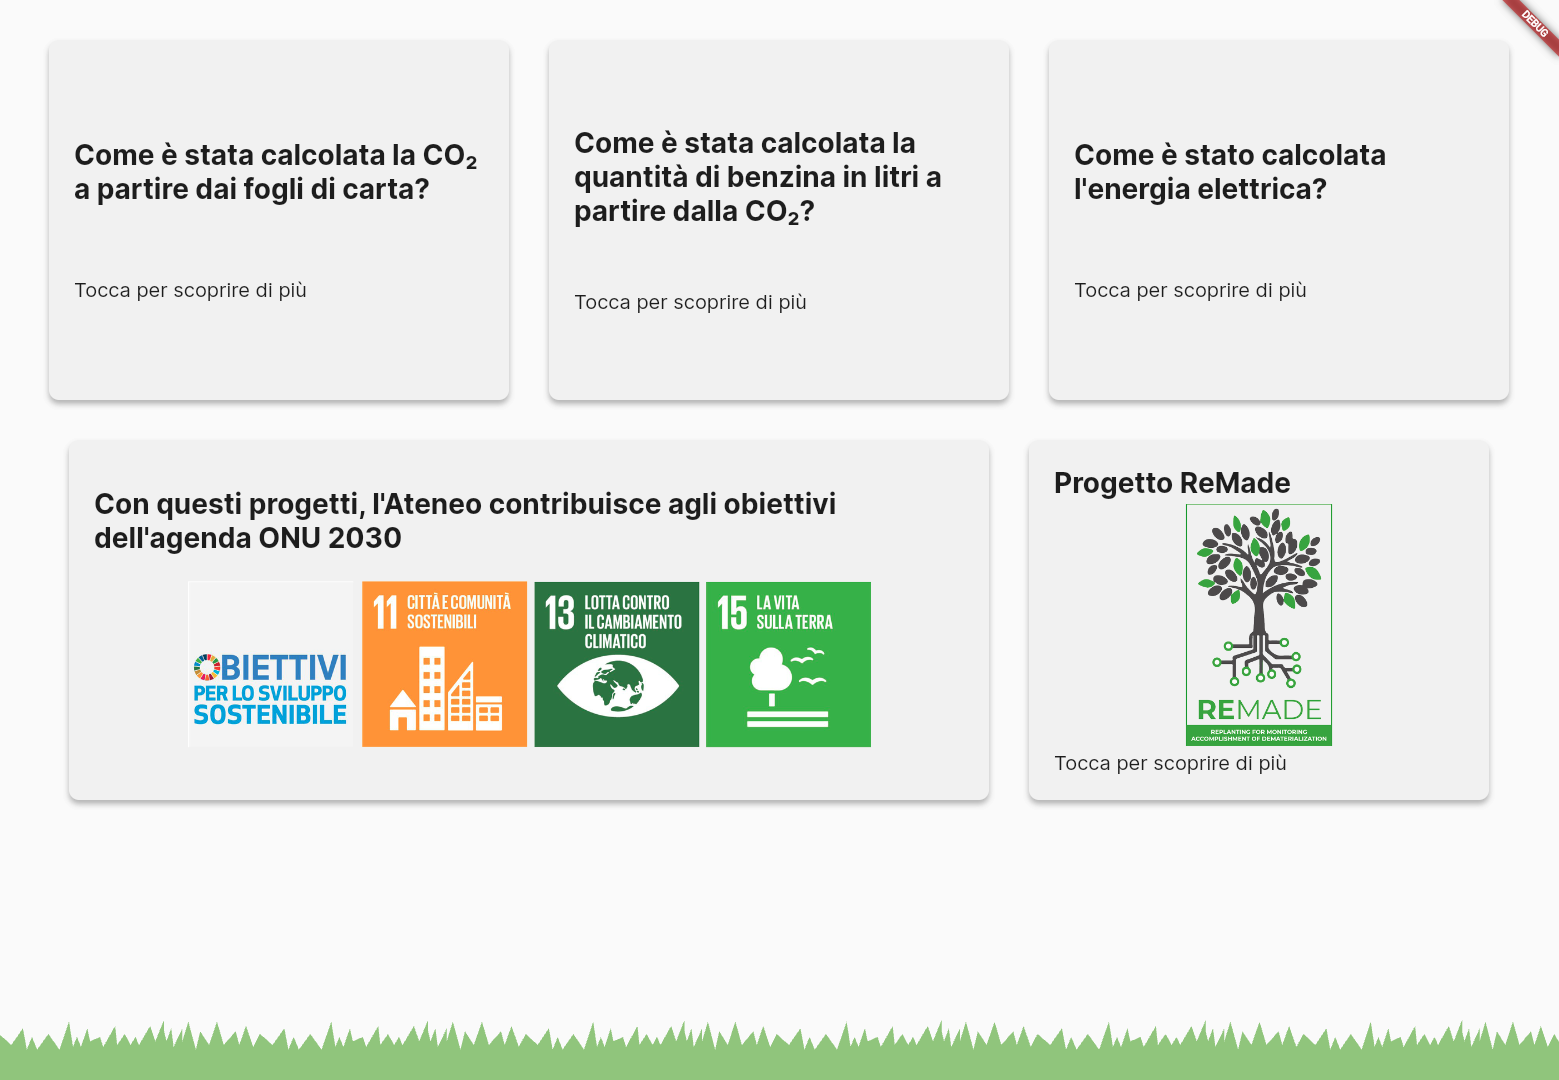
\includegraphics[width=\textwidth]{img/totem/screenshot/infoPageScreen.png}
    \caption{Pagina delle informazioni}
    \label{fig:infoPage}
  \end{minipage}
  \vfill
  \vspace{0.2 cm}
  \centering
  \begin{minipage}[h]{\linewidth}
    \centering
    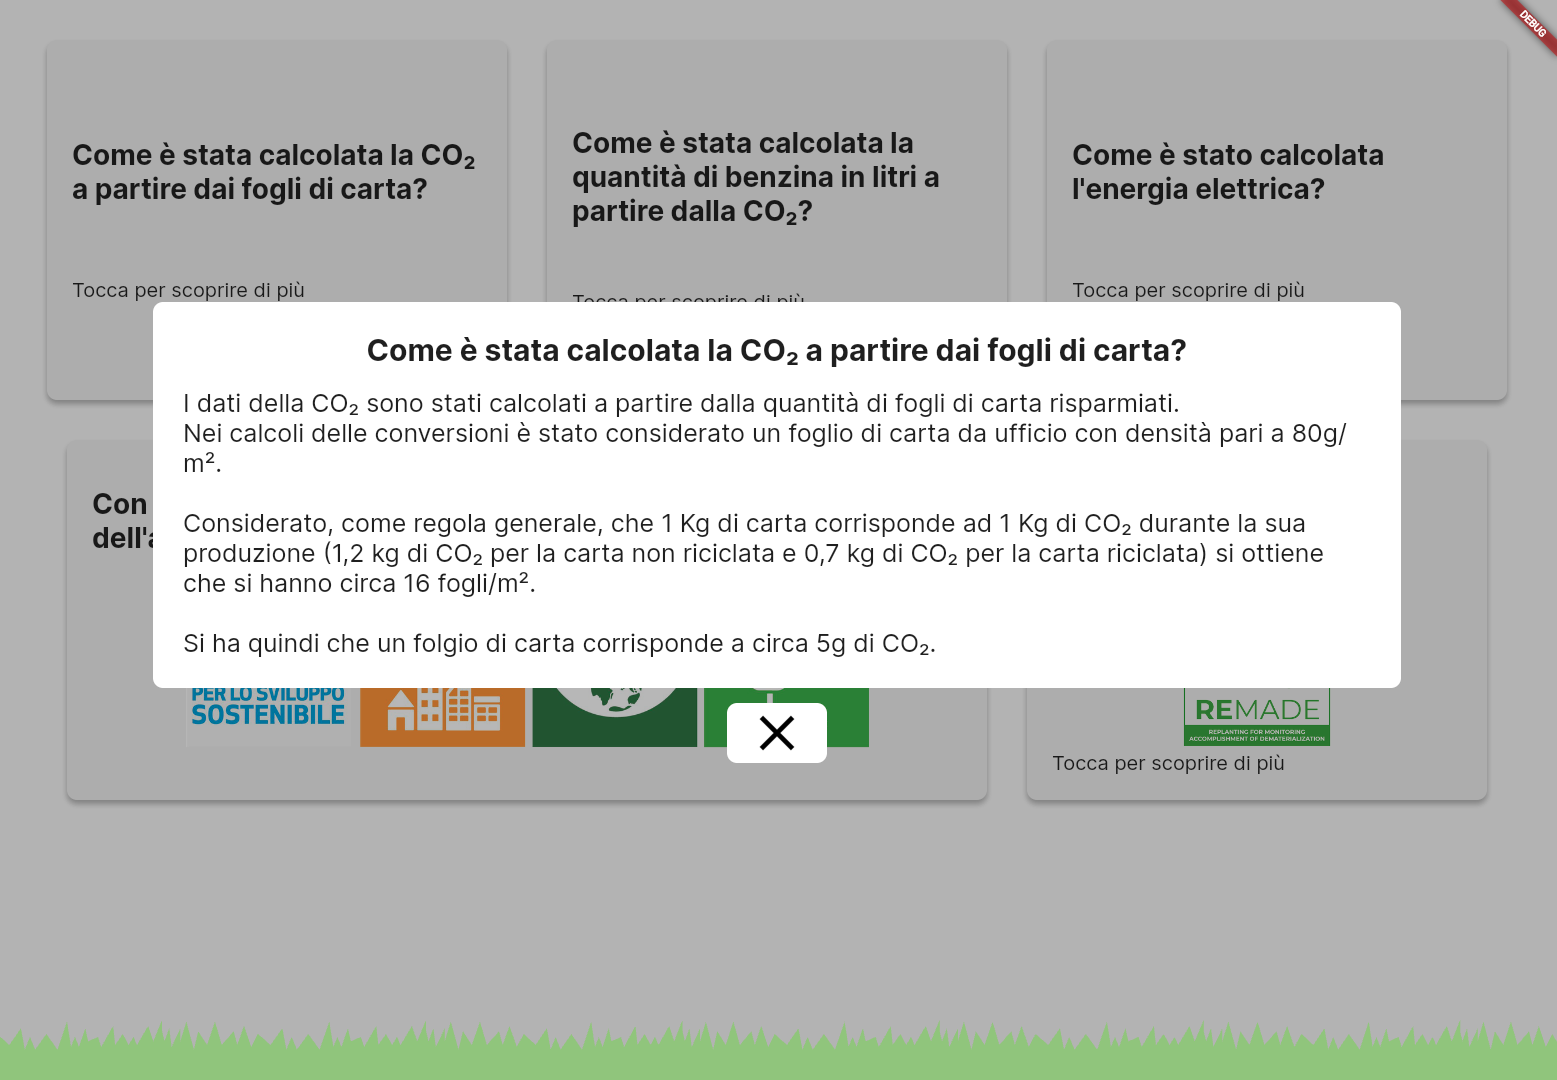
\includegraphics[width=0.9\textwidth]{img/totem/screenshot/infoPagePopupScreen.png}
    \caption{Pagina delle informazioni: tile selezionata espansa che mostra maggiori dettagli.}
    \label{fig:infoPagePopup}
  \end{minipage}
\end{figure}
